\documentclass[
  a4paper,
  oneside,
  BCOR = 10mm,
  DIV = 12,
  12pt,
  headings = normal,
]{scrartcl}

%%% Length calculations
\usepackage{calc}
%%%

%%% Support for color
\usepackage{xcolor}
\definecolor{lightblue}{HTML}{03A9F4}
\definecolor{red}{HTML}{F44336}
%%%

%%% Including graphics
\usepackage{graphicx}
%%%

%%% Font selection
\usepackage{fontspec}

\setromanfont{STIX Two Text}[
  SmallCapsFeatures = {LetterSpace = 8},
]

\setsansfont{IBM Plex Sans}[
  Scale = MatchUppercase,
]

\setmonofont{IBM Plex Mono}[
  Scale = MatchUppercase,
]
%%%

%%% Math typesetting
\usepackage{amsmath}

\usepackage{unicode-math}
\setmathfont{STIX Two Math}

\usepackage{IEEEtrantools}
%%%

%%% List settings
\usepackage{enumitem}
\setlist[enumerate]{
  label*      = {\arabic*.},
  left        = \parindent,
  topsep      = 0\baselineskip,
  parsep      = 0\baselineskip,
  noitemsep, % override itemsep
}
% List settings for levels 2–4
\setlist[enumerate, 2, 3, 4]{
  label*      = {\arabic*.},
  left        = 0em,
  topsep      = 0\baselineskip,
  parsep      = 0\baselineskip,
  noitemsep, % override itemsep
}

\setlist[itemize]{
  label*      = {—},
  left        = \parindent,
  topsep      = 0\baselineskip,
  parsep      = 0\baselineskip,
  itemsep     = 1\baselineskip,
  noitemsep, % override itemsep
}

\setlist[description]{
  font        = {\rmfamily\upshape\bfseries},
  topsep      = 1\baselineskip,
  parsep      = 0\baselineskip,
  itemsep     = 0\baselineskip,
}

%%%

%%% Structural elements typesetting
\setkomafont{pagenumber}{\rmfamily\upshape}
\setkomafont{disposition}{\rmfamily\bfseries}

% Sectioning
\RedeclareSectionCommand[
  beforeskip = -1\baselineskip,
  afterskip  = 1\baselineskip,
  font       = {\normalsize\bfseries\scshape},
]{section}

\RedeclareSectionCommand[
  beforeskip = -1\baselineskip,
  afterskip  = 1\baselineskip,
  font       = {\normalsize\bfseries\itshape},
]{subsection}

\RedeclareSectionCommand[
  beforeskip = -1\baselineskip,
  afterskip  = 1\baselineskip,
  font       = {\normalsize\bfseries},
]{subsubsection}

\RedeclareSectionCommand[
  beforeskip = -1\baselineskip,
  afterskip  = -0.5em,
  font       = {\normalsize\mdseries\scshape\addfontfeatures{Letters = {UppercaseSmallCaps}}},
]{paragraph}
%%%

%%% Typographic enhancements
\usepackage{microtype}
%%%

%%% Language-specific settings
\usepackage{polyglossia}
\setmainlanguage{ukrainian}
\setotherlanguages{english}
%%%

%%% Captions
\usepackage{caption}
\usepackage{subcaption}

%\DeclareCaptionLabelFormat{closing}{#2)}
%\captionsetup[subtable]{labelformat = closing}

%\captionsetup[subfigure]{labelformat = closing}

\captionsetup[table]{
  aboveskip = 0\baselineskip,
  belowskip = 0\baselineskip,
}

\captionsetup[figure]{
  aboveskip = 1\baselineskip,
  belowskip = 0\baselineskip,
}

\captionsetup[subfigure]{
  labelformat = simple,
  labelformat = brace,
  justification = RaggedRight,
  singlelinecheck = false,
}
%%%

%%% Hyphenated ragged typesetting
\usepackage{ragged2e}
%%%

%%% Table typesetting
\usepackage{booktabs}
\usepackage{longtable}

\usepackage{multirow}

\usepackage{array}
\newcolumntype{v}[1]{>{\RaggedRight\arraybackslash\hspace{0pt}}p{#1}}
\newcolumntype{b}[1]{>{\Centering\arraybackslash\hspace{0pt}}p{#1}}
\newcolumntype{n}[1]{>{\RaggedLeft\arraybackslash\hspace{0pt}}p{#1}}
%%%

%%% Drawing
\usepackage{tikz}
\usepackage{tikzscale}
\usetikzlibrary{datavisualization}
\usetikzlibrary{datavisualization.formats.functions}
\usetikzlibrary{positioning}
\usetikzlibrary{patterns}
\usetikzlibrary{intersections}
\usetikzlibrary{arrows.meta} % Stealth arrow tips

\usepackage{pgfplots}
\usepgfplotslibrary{fillbetween}
%%%

%%% SI units typesetting
\usepackage{siunitx}
\sisetup{
  output-decimal-marker = {,},
  exponent-product      = {\cdot},
  inter-unit-product    = \ensuremath{{} \cdot {}},
  per-mode              = symbol,
}
%%%

% Code Highlighting
\usepackage{minted}
\setmintedinline{
  style = bw,
  breaklines,
}

\newminted[bashterm]{text}{%
  autogobble,%
  breaklines,%
  style=bw,%
}

\newminted[codegeneric]{text}{%
  autogobble,%
  style=bw,%
  breaklines,%
  fontsize=\small,%
}

\newmintinline{bash}{%
}

\newmintinline[minttext]{text}{%
  breaklines,%
  breakanywhere,%
}

%%% Framing code listings
\usepackage{tcolorbox}
\tcbuselibrary{breakable}
\tcbuselibrary{minted}
\tcbuselibrary{skins}

% Text file listing
\newtcblisting[
  auto counter,
  list inside,
  number within = section,
]{listingplaintext}[3][]{%
  minted language = text,
  minted style    = bw,
  minted options  = {
    autogobble,
    linenos,
    tabsize = 4,
    breaklines,
    breakanywhere,
    fontsize = \footnotesize,
  },
  empty,
  sharp corners,
  coltitle = black,
  borderline horizontal = {1pt}{0pt}{black},
  titlerule = {0.5pt},
  titlerule style = {
    black,
  },
  toptitle = 0.3em,
  bottomtitle = 0.3em,
  before skip      = \intextsep,
  after  skip      = \intextsep,
  title            = {Лістинг \thetcbcounter: #2},
  list entry       = {\protect\numberline{\thetcbcounter}#2},
  left = 0em,
  right = 0em,
  %
  listing only,
  breakable,
  %
  label = {#3},%
}

\newtcbinputlisting[
  use counter from = listingplaintext,
  list inside,
  number within = section
]{\inputplaintext}[4][]{%
  minted language = text,
  minted style    = bw,
  minted options  = {
    autogobble,
    linenos,
    tabsize = 4,
    breaklines,
    breakanywhere,
    fontsize = \footnotesize,
  },
  empty,
  sharp corners,
  coltitle = black,
  borderline horizontal = {1pt}{0pt}{black},
  titlerule = {0.5pt},
  titlerule style = {
    black,
  },
  toptitle = 0.3em,
  bottomtitle = 0.3em,
  before skip      = \intextsep,
  after  skip      = \intextsep,
  title            = {Лістинг \thetcbcounter: #3},
  list entry       = {\protect\numberline{\thetcbcounter}#3},
  left = 0em,
  right = 0em,
  %
  listing file={#2},
  listing only,
  breakable,
  %
  label = {#4}
}

\newtcblisting[
  use counter from = listingplaintext,
  list inside,
  number within = section,
]{listingpython}[3][]{%
  minted language = python,
  minted style    = bw,
  minted options  = {
    autogobble,
    linenos,
    tabsize = 4,
    breaklines,
    breakanywhere,
    fontsize = \footnotesize,
  },
  empty,
  sharp corners,
  coltitle = black,
  borderline horizontal = {1pt}{0pt}{black},
  titlerule = {0.5pt},
  titlerule style = {
    black,
  },
  toptitle = 0.3em,
  bottomtitle = 0.3em,
  before skip      = \intextsep,
  after  skip      = \intextsep,
  title            = {Лістинг \thetcbcounter: #2},
  list entry       = {\protect\numberline{\thetcbcounter}#2},
  left = 0em,
  right = 0em,
  %
  listing only,
  breakable,
  %
  label = {#3},
  %
  #1%
}

\newtcbinputlisting[
  use counter from = listingplaintext,
  list inside,
  number within = section
]{\inputpython}[4][]{%
  minted language = python,
  minted style    = bw,
  minted options  = {
    autogobble,
    linenos,
    tabsize = 4,
    breaklines,
    breakanywhere,
    fontsize = \footnotesize,
  },
  empty,
  sharp corners,
  coltitle = black,
  borderline horizontal = {1pt}{0pt}{black},
  titlerule = {0.5pt},
  titlerule style = {
    black,
  },
  toptitle = 0.3em,
  bottomtitle = 0.3em,
  before skip      = \intextsep,
  after  skip      = \intextsep,
  title            = {Лістинг \thetcbcounter: #3},
  list entry       = {\protect\numberline{\thetcbcounter}#3},
  left = 0em,
  right = 0em,
  %
  listing file={#2},
  listing only,
  breakable,
  %
  label = {#4}
}

% Linux command-line listing
\newtcblisting{linuxterm}%
{%
  % Syntax highlighing options
  listing only,%
  minted language = bash,%
  minted options={%
    autogobble,%
    linenos%
  },%
  % Presentation options
  empty,%
  %% Margins
  sharp corners,%
  toptitle = 0.0em,%
  bottomtitle = 0.0em,%
  left = 0em,%
  right = 0em,%
  before skip = \intextsep,%
  after skip = \intextsep,%
}

\newtcblisting{linuxtermout}%
{%
  % Syntax highlighing options
  listing only,%
  minted language = text,%
  minted options={%
    autogobble,%
    linenos%
  },%
  % Presentation options
  empty,%
  %% Margins
  sharp corners,%
  toptitle = 0.0em,%
  bottomtitle = 0.0em,%
  left = 0em,%
  right = 0em,%
  before skip = \intextsep,%
  after skip = \intextsep,%
}

% Dockerfile listings
\newtcblisting[
  use counter from = listingplaintext,
  list inside,
  number within = section,
]{listingdocker}[3][]{%
  minted language = dockerfile,
  minted style    = bw,
  minted options  = {
    autogobble,%
    linenos,
    tabsize = 4,
    breaklines,
    breakanywhere,
    fontsize = \footnotesize,
  },
  empty,
  sharp corners,
  coltitle = black,
  borderline horizontal = {1pt}{0pt}{black},
  titlerule = {0.5pt},
  titlerule style = {
    black,
  },
  toptitle = 0.3em,
  bottomtitle = 0.3em,
  before skip      = \intextsep,
  after  skip      = \intextsep,
  title            = {Лістинг \thetcbcounter: #2},
  list entry       = {\protect\numberline{\thetcbcounter}#2},
  left = 0em,
  right = 0em,
  %
  listing only,
  breakable,
  %
  label = {#3},%
}

% Docker Compose listings
\newtcblisting[
  use counter from = listingplaintext,
  list inside,
  number within = section,
]{listingdockercompose}[3][]{%
  minted language = yaml,
  minted style    = bw,
  minted options  = {
    autogobble,%
    linenos,
    tabsize = 4,
    breaklines,
    breakanywhere,
    fontsize = \footnotesize,
  },
  empty,
  sharp corners,
  coltitle = black,
  borderline horizontal = {1pt}{0pt}{black},
  titlerule = {0.5pt},
  titlerule style = {
    black,
  },
  toptitle = 0.3em,
  bottomtitle = 0.3em,
  before skip      = \intextsep,
  after  skip      = \intextsep,
  title            = {Лістинг \thetcbcounter: #2},
  list entry       = {\protect\numberline{\thetcbcounter}#2},
  left = 0em,
  right = 0em,
  %
  listing only,
  breakable,
  %
  label = {#3},%
}


% Customize minted line numbers
\renewcommand{\theFancyVerbLine}{\ttfamily\scriptsize\arabic{FancyVerbLine}}

%%%

%%% Typeset menus and keys
\usepackage{menukeys}[
  os=win,
]
%%%

%%% Links and hyperreferences
\usepackage{hyperref}
\hypersetup{
  bookmarksnumbered = true,
  colorlinks      = false,
  linkbordercolor = red,
  urlbordercolor  = lightblue,
  pdfborderstyle  = {/S/U/W 1.5},
}
%%%

%%% Length adjustment

% Set baselineskip, default is 14.5 pt
\linespread{1.068966} % ~15.5 pt
\setlength{\emergencystretch}{1em}
\setlength{\parindent}{1.5em}
\newlength{\gridunitwidth}
\setlength{\gridunitwidth}{\textwidth / 12}
%%%

%%% Custom commands
\newcommand{\allcaps}[1]{%
  {%
    \addfontfeatures{%
      Letters = UppercaseSmallCaps,
      LetterSpace = 8,%
    }%
    #1%
  }%
}
\newcommand{\filename}[1]{\texttt{#1}}
\newcommand{\progname}[1]{\texttt{#1}}
\newcommand{\commandname}[1]{\texttt{#1}}
\newcommand{\modulename}[1]{\texttt{#1}}
\newcommand{\transeng}[1]{{англ.}~\textit{\textenglish{#1}}}
%%%

%%% Custom math commands
\newcommand{\longvar}[1]{\mathit{#1}}
\newcommand{\vect}[1]{\mathbfit{#1}}
\newcommand{\matr}[1]{\mathbfit{#1}}

\newcommand{\logequiv}{\mathrel{\Longleftrightarrow}} % Logically equivalent

\DeclareMathOperator*{\minimize}{min} % minimize for linear programs
%%%

\begin{document}

\begin{titlepage}
    \begin{center}
      Міністерство освіти і~науки України\\
      Національний авіаційний університет\\
      Факультет кібербезпеки, комп'ютерної та~програмної інженерії\\
      Кафедра комп'ютеризованих систем управління

      \vspace{\fill}
        Лабораторна робота №~1.3\\
        з~дисципліни «Дослідження операцій»\\
        на~тему «Симплексний метод розв'язку задачі лінійного програмування. Метод штучного базису»

      \vspace{\fill}

      \begin{flushright}
        Виконала:\\
        студентка \allcaps{ФККПІ}\\
        групи \allcaps{СП}-425\\
        Ульчич І.\,Г.\\
        Перевірила:\\
        Яковенко Л.\,В.
      \end{flushright}

      Київ 2019
    \end{center}
  \end{titlepage}

  \section{Завдання роботи}
    Розв'язати задачу лінійного програмування:
    \begin{IEEEeqnarray*}{l}
      L = -4 x_{1} - 3 x_{2} + 2 x_{3} \to \max,\\
      \left\{ \,
        \begin{IEEEeqnarraybox}[
          \IEEEeqnarraystrutmode
          \IEEEeqnarraystrutsizeadd{2pt}{2pt}
        ][c]{l}
             x_{2} + x_{3} \geqslant 1, \\
          -x_{1} + 2 x_{2} \leqslant 5, \\
             -2 x_{1} + 4 x_{2} - x_{3} = 1, \quad
            x_{1} \geqslant 0, \quad
            x_{2} \geqslant 0, \quad
            x_{3} \geqslant 0.
        \end{IEEEeqnarraybox}
      \right.
    \end{IEEEeqnarray*}

  \section{Хід~роботи}
    Щоб~розв'язати поставлену задачу симплексним методом, спочатку треба звести її~до~матричного вигляду. Нехай~$\vect{c}$~— вектор коефіцієнтів при~керованих змінних у~цільовій функції, $\matr{A_{\textbf{ub}}}$~— матриця коефіцієнтів при~керованих змінних у~нерівностях обмежень зверху, $\vect{x}$~— вектор керованих змінних, $\vect{b_{\textbf{ub}}}$~— вектор вільних членів при~нерівностях обмежень зверху, $\matr{A_{\textbf{eq}}}$~— матриця коефіцієнтів при~керованих змінних у~рівняннях обмежень, $\vect{b_{\textbf{eq}}}$~— вектор вільних членів при~рівняннях обмежень, $\vect{l}$~— вектор обмежень керованих змінних знизу, $\vect{u}$~— вектор обмежень керованих змінних зверху. Тоді задачу лінійного програмування можна представити так:
    \begin{IEEEeqnarray*}{l}
      \minimize_{\vect{x}} \vect{c}^{T} \vect{x}, \quad
        \text{враховуючи такі обмеження:} \quad
        \matr{A_{\textbf{ub}}} \vect{x} \leqslant \vect{b_{\textbf{ub}}},\,
        \matr{A_{\textbf{eq}}} \vect{x} = \vect{b_{\textbf{eq}}},\,
        \vect{l} \leqslant \vect{x} \leqslant \vect{u}.
    \end{IEEEeqnarray*}

    Так як у загальному вигляді задача лінійного програмування має на увазі мінімізацію, а за умовою дана задача максимізації, то перетворимо дану задачу максимізації~$L$ в еквівалентну задачу мінімізації~$L'$. Для цього досить помножити коефіцієнти цільової функції задачі~$L$ на~$-1$. Тоді оптимальні розв'язки еквівалентної задачі мінімізації~$L'$ при цільовому значенні~$-z$ будуть оптимальними розв'язками задачі максимізації~$L$ при цільовому значенні~$z$. Отже, цільова функція для еквівалентної задачі мінімізації~$L'$ виглядатиме так:
    \begin{IEEEeqnarray*}{rCl}
      L' &=& {-L(x)}
       =  -(-4 x_{1} - 3 x_{2} + 2 x_{3})
       =  4 x_{1} + 3 x_{2} - 2 x_{3}.
    \end{IEEEeqnarray*}

    Крім цього, одне з~обмежень~— нерівність виду~$\vect{a} \vect{x} \geqslant b$, приведемо її~до~вигляду~$\vect{a} \vect{x} \leqslant b$. Для~цього помножимо обидві частини нерівності~$x_{2} + x_{3} \geqslant 1$ на~$-1$, змінимо знак і~отримаємо нерівність $-x_{2} -x_{3} \leqslant -1$. Тоді маємо задачу:
    \begin{IEEEeqnarray*}{l}
      L' = 4 x_{1} + 3 x_{2} + -2 x_{3} \to \min,\\
      \left\{ \,
        \begin{IEEEeqnarraybox}[
          \IEEEeqnarraystrutmode
          \IEEEeqnarraystrutsizeadd{2pt}{2pt}
        ][c]{rCrCrCl}
           0 x_{1} &+& -1 x_{2} &+& -1 x_{3} &\leqslant& -1, \\
          -1 x_{1} &+&  2 x_{2} &+&  0 x_{3} &\leqslant& 5, \\
          -2 x_{1} &+&  4 x_{2} &+& -1 x_{3} &=& 1, \\
          \multicolumn{7}{l}{$0 \leqslant x_{i} \leqslant \infty, \quad i \in \{1, 2, 3\}.$}
        \end{IEEEeqnarraybox}
      \right.
    \end{IEEEeqnarray*}
    Запишемо задачу у~матричному представленні:
    \begin{IEEEeqnarray*}{rCl'rCl'rCl'rCl}
      \vect{c} &=& (4, 3, -2) &
      \matr{A_{\textbf{ub}}} &=&
      \begin{pmatrix}
         0 & -1 & -1 \\
        -1 &  2 &  0
      \end{pmatrix} &
      \vect{b_{\textbf{ub}}} &=&
      \begin{pmatrix}
        -1 \\
        5
      \end{pmatrix} &
      \vect{l} &=&
      \begin{pmatrix}
        0 & 0 & 0
      \end{pmatrix} \\
      %
      & & &
      \matr{A_{\textbf{eq}}} &=&
      \begin{pmatrix}
        -2 & 4 & -1
      \end{pmatrix} &
      \vect{b_{\textbf{eq}}} &=&
      \begin{pmatrix}
        1
      \end{pmatrix} &
      \vect{u} &=&
      \begin{pmatrix}
        \infty & \infty & \infty
      \end{pmatrix}
    \end{IEEEeqnarray*}
    Отримане матричне представлення подає умову задачі у~вигляді, зручному для~програмного роз\-в'\-я\-за\-ння~симплекс-методом. Отримавши зручне представлення умови задачі, розробляємо програму, яка~розв'яже~поставлену задачу~(лістинг~\ref{lst:01-solver-src}), і~запускаємо її~(рис.~\ref{fig:01-solver-res}).

    \begin{figure}[!htbp]
      \centering
      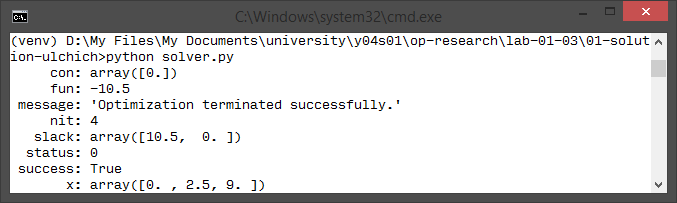
\includegraphics[width = \columnwidth]{./assets/p01.png}
      \caption{Результат розв'язання задачі програмою}
      \label{fig:01-solver-res}
    \end{figure}

    В~результаті бачимо, як~розроблена програма розв'язала поставлену задачу. Розв'язки наведені у рядку~\verb|x: array([0. , 2.5, 9.])|. Це означає, що оптимальними розв'язками є такий набір значень: $(x_{1} = 0, x_{2} = \num{2.5}, x_{3} = 9)$. При таких значеннях керованих змінних цільова функція еквівалентної задачі мінімізації набуває значення~$L'(\vect{x}) = z = \num{-10.5}$. Отже, значення цільової функції для початкової задачі максимізації~$L$ при знайдених значеннях буде дорівнювати~$L(\vect{x}) = -z = \num{10.5}$.

  \section{Висновок}
    Виконуючи дану лабораторну роботу, ми~навчились використовувати симплекс-метод для~розв'язання задач лінійного програмування, а~також розробляти програмне забезпечення для~допомоги при~розв'язанні задачі лінійного програмування симплекс-методом.

  \appendix
  \section{Програма для~розв'язку поставленої задачі}
    \inputpython{../01-solution-ulchich/solver.py}{Початковий код~програми для~розв'язання поставленої задачі лінійного програмування симплекс-методом}{lst:01-solver-src}

    \inputplaintext{../01-solution-ulchich/requirements.txt}{Файл з~описом залежностей розробленої програми}{lst:02-solver-requirements}

\end{document}
